\documentclass{oci}
\usepackage[utf8]{inputenc}
\usepackage{lipsum}
\usepackage{tikz}
\usetikzlibrary{patterns}

\title{Cubitos}

\begin{document}
\begin{problemDescription}

El pequeño Nelman es un niño muy alegre y pasa sus tardes recortando cubitos de papel y pegándolos como en la imagen siguiente:

\begin{center}
	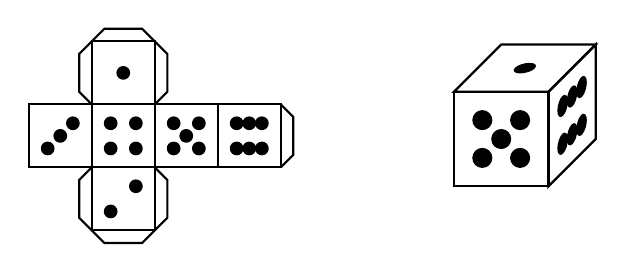
\begin{tikzpicture}[scale = 0.8]
\draw[thick] (0,0) rectangle +(1,1);
\draw[thick] (1,1) rectangle +(1,1);
\draw[thick] (1,0) rectangle +(1,1);
\draw[thick] (1,-1) rectangle +(1,1);
\draw[thick] (2,0) rectangle +(1,1);
\draw[thick] (3,0) rectangle +(1,1);
\draw[thick] (2,-1) -- (2.2,-0.8) -- (2.2,-0.2)-- (2,0);
\draw[thick] (1,-1) -- (1.2,-1.2) -- (1.8,-1.2)-- (2,-1);
\draw[thick] (1,-1) -- (0.8,-0.8) -- (0.8,-0.2)-- (1,0);
\begin{scope}[shift ={(0,2)}]
\draw[thick] (1,-1) -- (0.8,-0.8) -- (0.8,-0.2)-- (1,0);
\end{scope}
\begin{scope}[shift ={(1,1)}]
\draw[thick] (0,1) -- (0.2,1.2) -- (0.8,1.2)-- (1,1);
\end{scope}
\begin{scope}[shift ={(0,2)}]
\draw[thick] (2,-1) -- (2.2,-0.8) -- (2.2,-0.2)-- (2,0);
\end{scope}
\begin{scope}[shift ={(2,1)}]
\draw[thick] (2,-1) -- (2.2,-0.8) -- (2.2,-0.2)-- (2,0);
\end{scope}
\begin{scope}[shift ={(0.5,0.5)}]
\draw[fill = black] (1,1) circle (0.1);
\draw[fill = black] (1-0.2,-1-0.2) circle (0.1);
\draw[fill = black] (1+0.2,-1+0.2) circle (0.1);

\draw[fill = black] (0.2,+0.2) circle (0.1);
\draw[fill = black] (0,0) circle (0.1);
\draw[fill = black] (-0.2,-0.2) circle (0.1);

\draw[fill = black] (1.2,0.2) circle (0.1);
\draw[fill = black] (0.8,0.2) circle (0.1);
\draw[fill = black] (1.2,-0.2) circle (0.1);
\draw[fill = black] (0.8,-0.2) circle (0.1);

\draw[fill = black] (2,0) circle (0.1);
\draw[fill = black] (2.2,0.2) circle (0.1);
\draw[fill = black] (1.8,0.2) circle (0.1);
\draw[fill = black] (2.2,-0.2) circle (0.1);
\draw[fill = black] (1.8,-0.2) circle (0.1);

\draw[fill = black] (3,0.2) circle (0.1);
\draw[fill = black] (3,-0.2) circle (0.1);
\draw[fill = black] (3.2,0.2) circle (0.1);
\draw[fill = black] (2.8,0.2) circle (0.1);
\draw[fill = black] (3.2,-0.2) circle (0.1);
\draw[fill = black] (2.8,-0.2) circle (0.1);
\end{scope}


%%El cubito

\begin{scope}[scale={1.5}, shift={(-1.5,-0.2)}]
\draw[thick] (6,0) rectangle +(1,1);
\begin{scope}[cm={1,0,0,1,(6.5,0.5)}]
\draw[thick] (-0.5,-0.5) rectangle +(1,1);
\draw[fill = black] (0,0) circle (0.1);
\draw[fill = black] (0.2,0.2) circle (0.1);
\draw[fill = black] (-0.2,0.2) circle (0.1);
\draw[fill = black] (0.2,-0.2) circle (0.1);
\draw[fill = black] (-0.2,-0.2) circle (0.1);
\end{scope}

\begin{scope}[cm={0.5,0.5,0,1,(7,0)}]
\draw[thick] (0,0) rectangle +(1,1);
\begin{scope}[shift ={(-2.5,0.5)}]
\draw[fill = black] (3,0.2) circle (0.1);
\draw[fill = black] (3,-0.2) circle (0.1);
\draw[fill = black] (3.2,0.2) circle (0.1);
\draw[fill = black] (2.8,0.2) circle (0.1);
\draw[fill = black] (3.2,-0.2) circle (0.1);
\draw[fill = black] (2.8,-0.2) circle (0.1);
\end{scope}

\end{scope}
\begin{scope}[cm={1,0,0.5,0.5,(6,1)}]
\draw[thick] (0,0) rectangle +(1,1);
\draw[fill = black] (0.5,0.5) circle (0.1);
\end{scope}


\end{scope}


\end{tikzpicture}

\end{center}

Nelman no solo disfruta de recortar sus cubitos, también ama pintar sus lados de colores. Por simplicidad, siempre pinta el cubito antes de recortar el papel.

Luego de hacer muchos cubitos de la manera anterior, Nelman se percata de algo misterioso: ¡hay maneras distintas de pintar el diagrama de papel que dan el mismo cubo! Por ejemplo, las dos coloraciones siguientes dan el mismo cubo:

	\begin{center}
	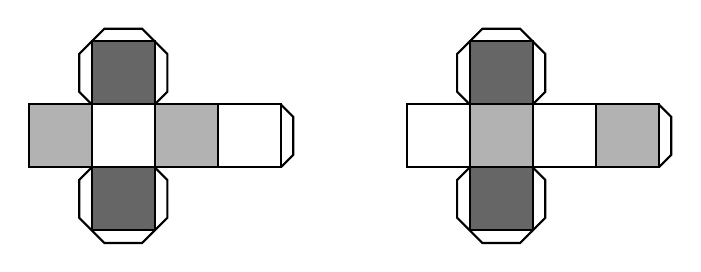
\begin{tikzpicture}[scale = 0.8]
	\draw[thick, fill=black!30] (0,0) rectangle +(1,1);
	\draw[thick, fill=black!60] (1,1) rectangle +(1,1);
	\draw[thick] (1,0) rectangle +(1,1);
	\draw[thick, fill=black!60] (1,-1) rectangle +(1,1);
	\draw[thick, fill=black!30] (2,0) rectangle +(1,1);
	\draw[thick] (3,0) rectangle +(1,1);
	\draw[thick] (2,-1) -- (2.2,-0.8) -- (2.2,-0.2)-- (2,0);
	\draw[thick] (1,-1) -- (1.2,-1.2) -- (1.8,-1.2)-- (2,-1);
	\draw[thick] (1,-1) -- (0.8,-0.8) -- (0.8,-0.2)-- (1,0);
	\begin{scope}[shift ={(0,2)}]
	\draw[thick] (1,-1) -- (0.8,-0.8) -- (0.8,-0.2)-- (1,0);
	\end{scope}
	\begin{scope}[shift ={(1,1)}]
	\draw[thick] (0,1) -- (0.2,1.2) -- (0.8,1.2)-- (1,1);
	\end{scope}
	\begin{scope}[shift ={(0,2)}]
	\draw[thick] (2,-1) -- (2.2,-0.8) -- (2.2,-0.2)-- (2,0);
	\end{scope}
	\begin{scope}[shift ={(2,1)}]
	\draw[thick] (2,-1) -- (2.2,-0.8) -- (2.2,-0.2)-- (2,0);
	\end{scope}
	
	\begin{scope}[shift ={(6,0)}]
	\draw[thick] (0,0) rectangle +(1,1);
	\draw[thick, fill=black!60] (1,1) rectangle +(1,1);
	\draw[thick, fill=black!30] (1,0) rectangle +(1,1);
	\draw[thick, fill=black!60] (1,-1) rectangle +(1,1);
	\draw[thick] (2,0) rectangle +(1,1);
	\draw[thick, fill=black!30] (3,0) rectangle +(1,1);
	\draw[thick] (2,-1) -- (2.2,-0.8) -- (2.2,-0.2)-- (2,0);
	\draw[thick] (1,-1) -- (1.2,-1.2) -- (1.8,-1.2)-- (2,-1);
	\draw[thick] (1,-1) -- (0.8,-0.8) -- (0.8,-0.2)-- (1,0);
	\begin{scope}[shift ={(0,2)}]
	\draw[thick] (1,-1) -- (0.8,-0.8) -- (0.8,-0.2)-- (1,0);
	\end{scope}
	\begin{scope}[shift ={(1,1)}]
	\draw[thick] (0,1) -- (0.2,1.2) -- (0.8,1.2)-- (1,1);
	\end{scope}
	\begin{scope}[shift ={(0,2)}]
	\draw[thick] (2,-1) -- (2.2,-0.8) -- (2.2,-0.2)-- (2,0);
	\end{scope}
	\begin{scope}[shift ={(2,1)}]
	\draw[thick] (2,-1) -- (2.2,-0.8) -- (2.2,-0.2)-- (2,0);
	\end{scope}
	\end{scope}
	
	\end{tikzpicture}
	\end{center}
	
De manera formal, diremos que dos cubitos son el mismo si existe alguna forma de rotarlos de modo tal que se vean idénticos. Puedes ayudar al pequeño Nelman a decidir si dos formas de colorear un diagrama producen el mismo cubito?

\end{problemDescription}

\begin{inputDescription}
Cada entrada consiste de dos líneas. Cada línea contiene $6$ números enteros $a_1$ $a_2$ $a_3$ $a_4$ $a_5$ $a_6$ entre el $0$ y el $5$, separados por un espacio, que codifican los colores de cada cubo. El orden de los colores es el detallado en la figura siguiente:


\begin{center}
	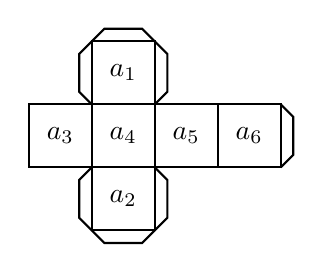
\begin{tikzpicture}[scale = 0.8]
	\draw[thick] (0,0) rectangle +(1,1);
	\draw[thick] (1,1) rectangle +(1,1);
	\draw[thick] (1,0) rectangle +(1,1);
	\draw[thick] (1,-1) rectangle +(1,1);
	\draw[thick] (2,0) rectangle +(1,1);
	\draw[thick] (3,0) rectangle +(1,1);
	\draw[thick] (2,-1) -- (2.2,-0.8) -- (2.2,-0.2)-- (2,0);
	\draw[thick] (1,-1) -- (1.2,-1.2) -- (1.8,-1.2)-- (2,-1);
	\draw[thick] (1,-1) -- (0.8,-0.8) -- (0.8,-0.2)-- (1,0);
	\begin{scope}[shift ={(0,2)}]
	\draw[thick] (1,-1) -- (0.8,-0.8) -- (0.8,-0.2)-- (1,0);
	\end{scope}
	\begin{scope}[shift ={(1,1)}]
	\draw[thick] (0,1) -- (0.2,1.2) -- (0.8,1.2)-- (1,1);
	\end{scope}
	\begin{scope}[shift ={(0,2)}]
	\draw[thick] (2,-1) -- (2.2,-0.8) -- (2.2,-0.2)-- (2,0);
	\end{scope}
	\begin{scope}[shift ={(2,1)}]
	\draw[thick] (2,-1) -- (2.2,-0.8) -- (2.2,-0.2)-- (2,0);
	\end{scope}
	\begin{scope}[shift ={(0.5,0.5)}]
	\node at (0,0) {$a_3$};
	\node at (1,0) {$a_4$};
	\node at (2,0) {$a_5$};
	\node at (3,0) {$a_6$};
	\node at (1,1) {$a_1$};
	\node at (1,-1) {$a_2$};
	\end{scope}
	\end{tikzpicture}
\end{center}

\end{inputDescription}

\begin{outputDescription}
La salida es un caracter $1$ si los cubos son iguales, o $0$ si son distintos.
\end{outputDescription}

\begin{scoreDescription}
  Este problema no contiene subtareas.
  Se evaluarán exactamente 200 casos de prueba y se otorgará puntaje de acuerdo a la cantidad de
  casos correctos.
  Si $C$ es la cantidad de casos correctos, el puntaje recibido será $\max(C-100,0)$. 
\end{scoreDescription}

\begin{sampleDescription}
\sampleIO{sample-1}
\sampleIO{sample-2}
\sampleIO{sample-3}
\end{sampleDescription}

\end{document}
